% 8185: Quant Ellen PS2

\documentclass[12pt]{article}
%\usepackage[T1]{fontenc}
%\usepackage{lipsum}
\renewcommand{\baselinestretch}{1.2} 
\usepackage{graphicx}
\usepackage{hyperref}
\hypersetup{
    colorlinks=true,
    urlcolor=blue,
    citecolor=blue
}
\usepackage[export]{adjustbox}
\usepackage{subcaption}
\usepackage{amsmath}
\usepackage{amsfonts}
\usepackage{geometry}
\setcounter{MaxMatrixCols}{20}
\geometry{a4paper,
 left=3cm,right=3cm,
 top=1.5cm, bottom=1.5cm}

\usepackage{natbib}
\bibliographystyle{apalike}

%\usepackage{natbib}
%setcitestyle{authoryear,open={(},close={)}}
\graphicspath{ {../figs/} }

\begin{document}
%\thispagestyle{myheadings}
%\markright{Indian Statistical Institute, New Delhi\hfill }

\title{Econ 8185: Quant PS2}
\author{Bipul Verma}
\date{\today}
\maketitle

%\tableofcontents{}
\abstract{The present document calculates  policy functions, of an economy with distortions.\footnote{Acknowledgement: Fran, Jacob, Maria.} We use two methods - LQ and Vaughan (with log linearization) to solve the model.}

\vspace{8cm}

%\begin{center}
%\includegraphics[scale=0.4]{isi_logo.png}
%\end{center}
%\begin{center}
%\begin{Large}
%INDIAN STATISTICAL INSTITUTE, NEW-DELHI.
%\end{Large}
%\end{center}


\newpage

\section{Model}
The growth model with distortions can be written in the following form after making substitutions from the government budget constraints and de trending the variables.

$$\max_{\hat{c}_t, h_t , \hat{k}_{t+1}} \sum \hat{\beta}^t U(\hat{c}_t, h_t)$$

subject to 
\begin{multline*}
(1+\tau_{ct})\hat{c}_t + (1-\tau_{dt})\hat{x}_t = (1-\tau_{dt})(r_t -\tau_{pt}(r_t -\delta))\hat{k}_t \\                                                 + (1-\tau_{ht})\hat{w}_th_t + \kappa_t
\end{multline*}

$$\tilde{\gamma} \hat{k}_{t+1} = (1-\delta)\hat{k}_t + \hat{x}_t$$

$$S_{t+1} = PS_t + \Sigma \epsilon_{t+1}$$ 

where $\hat{a} = \frac{a}{(1+\gamma_z)^t}$ variables denotes the de-trended variables with respect to productivity growth, $\tilde{\gamma} = (1+\gamma_n)(1+\gamma_z)$, $U(c, h) = log(c) + \psi log(1-h)$, $S_t = [log(z_t), \tau_{ct}, \tau_{ht}, \tau_{dt}, \tau_{pt}, log(g_t)]'$. 

\subsection{Parameters}
The parameter values are taken from Franciso Bullano's HW2 which are based on Bhandari, McGrattan \& Yao (2020). Same parameters will act as a check for the final answers. 


\begin{center}
\begin{table}[h]
\centering
\begin{tabular}{| c | c | c | c | }
\hline
\textbf{Parameters} & \textbf{Value} & \textbf{Parameters} & \textbf{Value} \\
\hline
$\beta$ & 0.95 & $\bar\tau_c$ & 0.065\\
\hline
$\delta$ & 0.05 & $\bar\tau_h$ & 0.38\\
\hline
$\psi$ & 1.6  &  $\bar\tau_d$ & 0.133\\
\hline
$\gamma_n$ & 0.02 & $\bar\tau_p$ & 0.36\\
\hline
$\gamma_z$ & 0.02 & $g_{share}$ & 0.17\\
\hline
$\theta$ & 0.34 & &\\
\hline
\end{tabular}
\caption{Parameter Selection}
\end{table}
\end{center}

\subsection{Specifying the AR(1) process}
An AR(1) stochastic process $\{z_t\}$ with mean $\mu_z$ and coefficient $\rho_z$ is written in the state space representation as:
\begin{align*}
	z_{t+1} = (1-\rho_z)\mu_z + \rho z_t + \epsilon_{t+1}, \; \; \; \; \epsilon\sim N(0, \sigma).
\end{align*}
As indicated by the Table 1, all the state variables have a non-zero mean in the present case. Hence, we have to augment the coefficient matrix appropriately. The law of motion for the state can then be specified as shown below.\footnote{Note that we have augmented the states with a constant 1.}
\begin{align*}
	\begin{bmatrix}
		1 \\log (z_{t+1}) \\ \tau_{ct+1} \\ \tau_{ht+1} \\ \tau_{dt+1} \\ \tau_{pt+1} \\ \log (g_{t+1})
	\end{bmatrix} = \begin{bmatrix}
		1 & 0 & 0 & 0 & 0 & 0 & 0 \\
		(1-\rho_z)\log ( \bar z) & \rho_z & 0 & 0 & 0 & 0 & 0 \\
		(1-\rho_{\tau c})\bar \tau_c & 0 & \rho_{\tau c} & 0 & 0 & 0 & 0 \\
		(1-\rho_{\tau h})\bar \tau_h & 0  & 0 & \rho_{\tau h} & 0 & 0 & 0 \\
		(1-\rho_{\tau d})\bar \tau_d & 0  & 0  & 0 & \rho_{\tau d} & 0 & 0 \\
		(1-\rho_{\tau p})\bar \tau_p & 0  & 0  & 0  & 0 & \rho_{\tau p} & 0 \\
		(1-\rho_{\tau g})\log (\bar g) & 0  & 0  & 0  & 0 & 0 &\rho_{g}\\
	\end{bmatrix} 	\begin{bmatrix}
		1 \\log (z_{t}) \\ \tau_{ct} \\ \tau_{ht} \\ \tau_{dt} \\ \tau_{pt} \\ \log (g_{t})
	\end{bmatrix} + \Sigma\epsilon_{t+1}
\end{align*}
Note: The value for $\bar g$ is obtained after calculating the steady state using the fact that $\bar g = (g_{share}) \bar y$.

\section{Steady State}
The following conditions characterize the consumers optimal choice:
\begin{align*}
\textbf{[MRS]:     } & \; \; \; \; \; \hspace{2mm}  \frac{-u_h(t)}{u_c(t)} = \frac{(1-\tau_{ht})\hat{w}_t}{(1+\tau_{ct})} \\
\textbf{[Euler]:     } & \; \; \; \; \; \frac{\tilde{\gamma} u_c(t) (1-\tau_{dt})}{(1+\tau_{ct})} = \frac{\hat{\beta} u_c(t+1)(1-\tau_{dt+1})}{1+\tau_{ct+1}}\Big[(r_{t+1} - \tau_{pt+1}(r_{t+1} -\delta)) + (1-\delta) \Big]  \\
\textbf{[Resource]: } & \; \; \; \; \;  \hat{c}_t + \tilde{\gamma} \hat{k}_{t+1} - (1-\delta)\hat{k}_t + \hat{g}_t = (\hat{k}_t)^{\theta}(z_t h_t)^{1-\theta}
\end{align*}

The MRS, and Euler equation along with the resource constraints forms a system of 3 equations in 3 variables at the steady state.
We solve the steady state values for two different specifications of the parameters. In the first specification we set all the taxes and transfers to zero and set parameter values same as in HW1.  The steady state of the de-trended variables is as follows: $\hat{k}_{ss} = 1.64011, h_{ss} = 0.354382, \hat{c}_{ss} = 0.4483689.$  The steady state value matches the HW1 values exactly. In the second specification all the taxes, transfers, parameters are set according to the parameters specified in Table 1. In this case the steady state values are  $\hat{k}_{ss} =  1.3253, h_{ss} = 0.322, \hat{c}_{ss} = 0.336.$

\section{LQ}
Note that \begin{multline*} \hat{c}_t = \frac{1}{1+ \tau_{ct}} \Big[r_t\hat{k}_t + \hat{w}_th_t + \hat{\kappa} -\tau_{ht}\hat{w}_th_t - \tau_{pt}(r_t - \delta)\hat{k}_t \\ -\tau_{dt}(r_t \hat{k}_t -\tau_{pt}(r_t -\delta)\hat{k}_t) -(1-\tau_{dt})\hat{x}_t \Big] 
\end{multline*}
where
\begin{align*}
\hat{w}_t(\hat{K}_t, H_t) & = (1-\theta)(\frac{\hat{K}_t}{H_t})^{\theta} (z_t)^{1-\theta}\\
r_t(\hat{K}_t, H_t) & = \theta (\hat{K}_t)^{\theta -1} (z_t H_t)^{1-\theta}\\
\hat{x}_t &= \tilde{\gamma}\hat{k}_{t+1} -(1-\delta)\hat{k}_t \\
\hat{X}_t & = \tilde{\gamma}\hat{K}_{t+1} -(1-\delta)\hat{K}_t \\
\hat{\kappa}_t & = \tau_{ct}\hat{C}_t + \tau_{ht}\hat{w}_tH_t + \tau_{pt}(r_t-\delta)\hat{K}_t + \tau_{dt}(r_t\hat{K}_t -\tau_{pt}\hat{K}_t(r_t -\delta))- \tau_{dt}\hat{X}_t - \hat{g}_t.
\end{align*}
Note that $\hat{K}_t, H_t$ represents the \textbf{aggregate per-capita} states in the sense that consumer can't influence them and takes these states as given.\footnote{Note that these aggregate per-capita variable are constructed just to ensure that they are taken as given by individual agent during optimization} In equilibrium $\hat{K}_t = \hat{k}_t, H_t = h_t$. 

Now define the vector of choice variables as $u_t$, the individual state variables as $X_{1t}$, the exogenous state variables as $X_{2t}$, and the aggregate state variables as $X_{3t}$. The content of these vectors are outlined below: \begin{align*}
	u_t = \begin{bmatrix}
		\hat{k}_{t+1} \\
		h_t
	\end{bmatrix}_{2 \times 1}, \; X_{1t} = \begin{bmatrix} 1 \\ k_t \end{bmatrix}_{2\times 1}, X_{2t} = \begin{bmatrix} S_t \end{bmatrix}_{7\times 1}, X_{3t} = \begin{bmatrix}
K_t \\ K_{t+1} \\ H_t 
\end{bmatrix}_{3 \times 1}. 
\end{align*}
All the state variables are stacked together in vector $X_t$ as shown below:
$$X_t = \begin{bmatrix} X_{1t} \\ X_{2t} \\ X_{3t} \end{bmatrix}_{12 \times 1}.$$

Thus we have been able to express $\hat{c}$ and hence utility in terms of choice variables $u$ and state variables $X$. The utility function to the problem can be written, after 2nd order Taylor expansion around the steady state as $$r(X, u) \approx  X'QX + u'Ru + 2X'Wu,$$ where $Q_{12 \times 12}$ , $R_{2 \times 2}$, and $W_{12 \times 2}$ are known matrices after the Taylor expansion. The optimal growth problem (with distortions) then reduced to solving the following: \begin{align*}
	\max_{u} \sum_t \hat\beta^t r(x_t, u_t) \\
	 \text{s.t. } X_{t+1} = A X_t + B u_t + C \epsilon_t .
\end{align*} The matrices $A, B, C$ can obtained by writing the constraints  in matrix form as follows:

\begin{multline*}
\begin{bmatrix} X_{1t+1} \\ X_{2t+1} \\ X_{3t+1} \end{bmatrix}_{12 \times 1} 
= \begin{bmatrix} [A_{11}]_{2 \times 2} & [A_{12}]_{2 \times 7} & [A_{13}]_{2 \times 3} \\
                  [0]_{7 \times 2} & [A_{22}]_{7 \times 7} & [A_{23}]_{7 \times 3} \\
                  [0]_{3 \times 2} & [A_{32}]_{3 \times 7} & [A_{33}]_{3 \times 3} \end{bmatrix} \begin{bmatrix} X_{1t} \\ X_{2t} \\ X_{3t} \end{bmatrix}_{12 \times 1} \\                  
                  + \begin{bmatrix} 0 & 0 \\ 1 & 0 \\ [0]_{10 \times 1} & [0]_{10 \times 1}\end{bmatrix}_{12 \times 2}
 \begin{bmatrix} k_{t+1} \\ h_t \end{bmatrix}_{2 \times 1}   + \mathbf{\Sigma \epsilon}
\end{multline*}
From the given problem $A_{11} = \begin{bmatrix} 1 & 0 \\ 0 & 0 \end{bmatrix}$, $A_{22} = [P]$ are known, while $A_{12}, A_{13}, A_{23}$ are matrices of zeros. We obtain matrices $\tilde{A}, \tilde{B}, \tilde{Q}$ as suggested in the notes. We finally obtain the following matrices which will be used later in the computation: 
\begin{equation*}
\tilde{A}_y = \begin{bmatrix} \tilde{A}_{11} & \tilde{A}_{12} \\ 0 & \tilde{A}_{22} \end{bmatrix}_{9 \times 9}; \tilde{A}_z = \begin{bmatrix} \tilde{A}_{13} \\ \tilde{A}_{23} \end{bmatrix}_{9 \times 3} 
\end{equation*}

We also make use of the market clearing conditions given by: $$X_{3t} = \Theta [X_{1t} X_{2t}]' + \Psi u_t.$$ For the current problem these matrices are given as:
 \begin{equation*}
\Theta = \begin{bmatrix} 0 & 1 & 0 & 0 & 0 & 0 & 0 & 0 & 0\\ 0 & 0 & 0 & 0 & 0 & 0 & 0 & 0 & 0\\ 0 & 0 & 0 & 0 & 0 & 0 &0 &0 & 0\end{bmatrix}_{3 \times 9}; \Psi = \begin{bmatrix} 0 & 0 \\ 1 & 0 \\ 0 & 1\end{bmatrix}
\end{equation*}

Once we have all the required matrices with us we can compute the policy functions using the formulas mentioned in the notes.
The policy functions are as follows: 
\begin{align*}
k'(.) &  =  0.123  +0.886k   +0.40\ln(z)  +0.182\tau_c  -0.438\tau_h   +0.538\tau_d    -0.039\tau_p   - 0.052 \ln(g)\\
h(.) & = 0.599   -0.046k  +0.149\ln(z)  -0.066\tau_c  -0.515\tau_h  +0.286\tau_d  -0.021\tau_p  +0.018\ln(g)
\end{align*}

\subsection{Results from LQ}
We plot the time series of capital, hours worked, and output based on the policy function obtained using LQ method below.
\begin{figure}[h]
    \centering
    \begin{minipage}{0.45\textwidth}
        \centering
        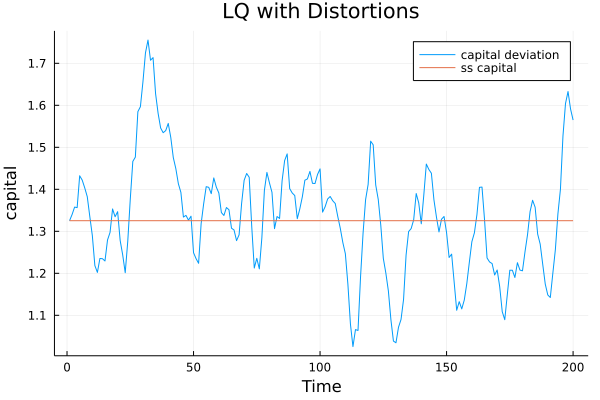
\includegraphics[width=1\textwidth]{k_dev_LQ_new.png} % first figure itself
        \caption{Capital deviation: LQ}\label{LQ_sim}
    \end{minipage}\hfill
    \begin{minipage}{0.45\textwidth}
        \centering
        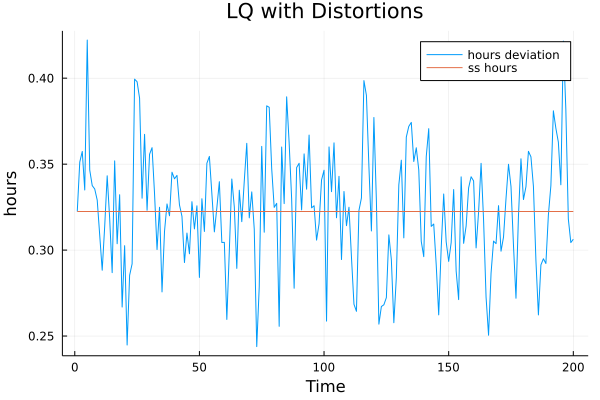
\includegraphics[width=1\textwidth]{h_dev_LQ_new.png} % second figure itself
        \caption{Hours deviation: LQ}\label{LQ_sim}
    \end{minipage}
        \begin{minipage}{0.45\textwidth}
        \centering
        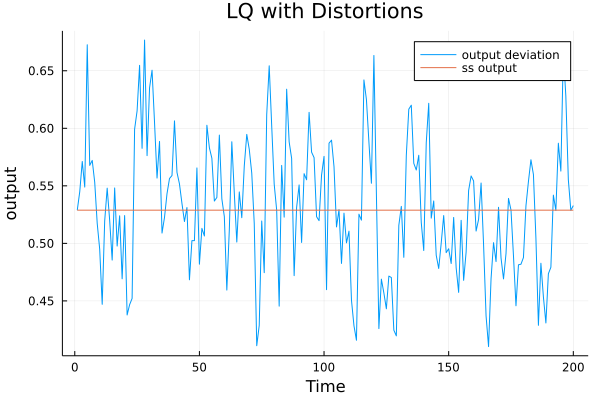
\includegraphics[width=1\textwidth]{y_dev_LQ_new.png} % first figure itself
        \caption{Output deviation: LQ}\label{LQ_sim}
    \end{minipage}\hfill
    \begin{minipage}{0.45\textwidth}
        \centering
        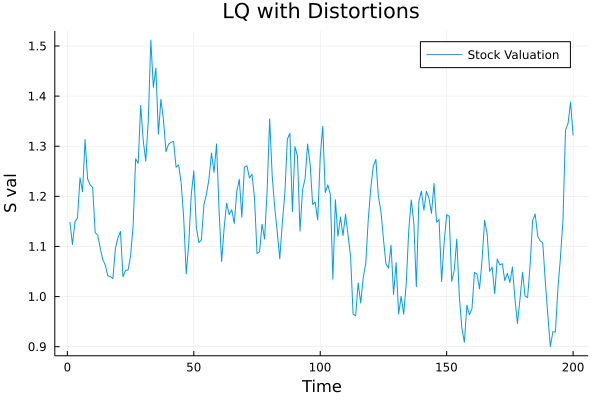
\includegraphics[width=1\textwidth]{stock_dev_LQ_new.png} % second figure itself
        \caption{Stock V deviation: LQ}\label{LQ_sim}
    \end{minipage}
\end{figure}


\section{Vaughan Method}
\subsection{Note on Linear RE Models}\label{note_RE}
Linear Approximation of FOCs usually leads us to the following system:
\begin{align*}
X_{t+1} = A_{xx}X_t + A_{xy}Y_t + \epsilon_{t+1}\\
\mathbf{E}[Y_{t+1}] = A_{yx} X_t + A_{yy}Y_t
\end{align*}
where $X_t$ denotes the endogenous state variable, $Y_t$ denotes the controls, and $\epsilon_t \sim N(0, Q)$. A RE (Rational Expectation) model assumes that one period forecast error is zero i.e  $X_{t+1} - \mathbf{E}[X_{t+1}] = \mathbf{E}[\epsilon_{t+1}] = 0.$ For the above system we are looking for a solution of the form:
\begin{align*}
X_{t+1} & = M X_t + \epsilon_{t+1} \\
Y_t & = C X_t .
\end{align*} 
Note that the above system is written in a \textit{state space} form. We want to make use of matrices $A_{xx}, A_{xy}, A_{yy}$ to get the matrices $M$, and $C$. Stacking together the system of FOCs can be written as:
\begin{align*}
\mathbf{E}\begin{bmatrix} X_{t+1} \\ Y_{t+1} \end{bmatrix} = \underbrace{\begin{bmatrix} A_{xx} & A_{xy} \\ A_{yx} & A_{yy}\end{bmatrix}}_A  \begin{bmatrix} X_{t} \\ Y_{t} \end{bmatrix}.
\end{align*}
The next step is to do a Schur decomposition of A. We can then rewrite A as:
\begin{align*}
A & = ZTZ^{-1} \\
T & = \begin{bmatrix} T_{\theta \theta} & T_{\theta \delta} \\ 0 & T_{\delta \delta} \end{bmatrix}.
\end{align*}
Here the diagonal elements of $T$ contains the eigenvalues and ordered in a manner such that $T_{\theta\theta}$ containing all stable eigenvalues ($|e| < 1$) with $Z$ contains the corresponding eigenvectors. Thus the linearized system of FOCs can be written as:
\begin{align*}
\mathbf{E}\begin{bmatrix} X_{t+1} \\ Y_{t+1} \end{bmatrix} & = ZTZ^{-1} \begin{bmatrix} X_{t} \\ Y_{t} \end{bmatrix} \\
Z^{-1}\mathbf{E}\begin{bmatrix} X_{t+1} \\ Y_{t+1} \end{bmatrix} & = TZ^{-1} \begin{bmatrix} X_{t} \\ Y_{t} \end{bmatrix}
\end{align*}
Now instead of keeping track of $X_t, Y_t$, we'll keep track of transformed variable $\theta_t, \delta_t$ as defined below and convert back as required.
\begin{align*}
\begin{bmatrix} \theta_t \\ \delta_t \end{bmatrix} & = Z^{-1} \begin{bmatrix} X_t \\ Y_t \end{bmatrix}.
\end{align*}
The linearized system then becomes:
\begin{align*}
\mathbf{E}\begin{bmatrix} \theta_{t+1} \\ \delta_{t+1} \end{bmatrix} & = T \begin{bmatrix} \theta_{t} \\ \delta_{t} \end{bmatrix} \\
\mathbf{E}\begin{bmatrix} \theta_{t+1} \\ \delta_{t+1} \end{bmatrix} & = \begin{bmatrix} T_{\theta \theta} & T_{\theta \delta} \\ 0 & T_{\delta \delta} \end{bmatrix} \begin{bmatrix} \theta_{t} \\ \delta_{t} \end{bmatrix}.
\end{align*}

Looking at the second set of equations:
\begin{align*}
\mathbf{E}[\delta_{t+1}] = T_{\delta\delta} \delta_t.
\end{align*}
Note that since $T_{\delta\delta}$ contains the unstable roots ($|e| > 1$), we require $\delta_t = 0$ for the solution to be stable. Now given $\delta_t = 0$, from the first set of equations we get, $\mathbf{E}[\theta_{t+1}] = T_{\theta\theta} \theta_t$. Note that:
\begin{align*}
\begin{bmatrix} X_t \\ Y_t \end{bmatrix} & = Z \begin{bmatrix} \theta_t \\ \delta_t \end{bmatrix} \\
\begin{bmatrix} X_t \\ Y_t \end{bmatrix} & = \begin{bmatrix} Z_{\theta x} & Z_{\delta x} \\ Z_{\theta y} & Z_{\delta y} \end{bmatrix} \begin{bmatrix} \theta_t \\ \delta_t \end{bmatrix}.
\end{align*}
Since $\delta_t =0$, we finally arrive at:
\begin{align*}
X_t = Z_{\theta x} \theta_t \\
Y_t = Z_{\theta y} \theta_t.
\end{align*}
Now going back to our initial system of equations:
\begin{align*}
\epsilon_{t+1} & = X_{t+1} - \mathbf{E}[X_{t+1}] \\
& = Z_{\theta x} \theta_{t+1} - Z_{\theta x} \mathbf{E}[\theta_{t+1}] \\
& = Z_{\theta x} (\theta_{t+1} - T_{\theta \theta} \theta_t).  
\end{align*}
If $Z_{\theta x}$ is invertible then the previous equation can be used to obtain the law of motion for $\theta_t$, which can then be used to derive the law of motion for $x_t$. It is not necessary that $Z_{\theta x}$ is invertible, it may not even be a square matrix. For $Z_{\theta x}$ to be invertible $n_{\theta} = n_{x}$, i.e the number of stable eigen-roots must equal the number of endogenous state variables. This is known as the \textit{Blanchard-Kahn condition}. In case $n_{\theta} < n_{x}$, we have no solution, $n_{\theta} > n_{x}$, we have infinite solutions to the system of equations. Suppose that the Blanchard-Kahn conditions hold. Then, from the last equation, we obtain the law of motion for $\theta_t$ as
\begin{align*}
\theta_{t+1} = T_{\theta\theta} \theta_t + Z_{\theta x}^{-1} \epsilon_{t+1}.
\end{align*}
Given $X_{t+1} = Z_{\theta x} \theta_{t+1}$, and $Y_t = Z_{y \theta} \theta_t$, we arrive at:
\begin{align*}
X_{t+1} & = \underbrace{Z_{\theta x} T_{\theta \theta}Z_{\theta x}^{-1} }_M X_t + \epsilon_{t+1} \\
Y_{t+1} & = \underbrace{Z_{\theta x} Z_{ \theta y }^{-1}}_C X_t.
\end{align*}
Thus, we finally have the required matrices as:
$$M =Z_{\theta x} T_{\theta \theta}Z_{\theta x}^{-1}, \; \; \; \; \;  C = Z_{ \theta y } Z_{\theta x}^{-1} .$$
Note that $M$, and $C$ are independent of $Q$. This is the CE (Certainty Equivalence) result in first order approximations. 

\subsection{Note on log-linearization}
Define the log deviation around steady state as: $$\tilde{x} = log(\frac{x}{x_{ss}}).$$ Then: 
\begin{gather*}
x = (x_{ss}) exp\{\tilde{x}\} \\
x \approx (x_{ss})(1+\tilde{x}) \\
\tilde{x} \approx \frac{x}{x_{ss}} -1.
\end{gather*}
Suppose we have the following equation with us which we want log-linearize around the steady state:\footnote{We have kept the variable as $x, \log(y)$ to outline that some stochastic varibles are AR(1) in logs while others in levels. }
\begin{align*}
F(x, \log (y)) = 0.
\end{align*}
The above equation can be rewritten in log-deviation form as follows:
\begin{align*}
G(\tilde{x}, \tilde{y}) = F((1+\tilde{x})x_{ss}, exp\{\tilde{y}\ }y_{ss}) = 0.
\end{align*}
To log-linearize, we simply take the first-order Taylor expansion of the above equation around $0$ to obtain:
\begin{align*}
G_{\tilde{x}}(.)\tilde{x} + G_{\tilde{y}}\tilde{y} = 0\\
(F_x(.)x_{ss}) \tilde{x} + (F_y(.)y_{ss})\tilde{y} = 0.
\end{align*} 


\subsection{Vaughan using Log Linearisation}
We start with the following first order condition that characterizes the equilibrium-
\begin{gather*}
 \frac{-u_h(t)}{u_c(t)} = \frac{(1-\tau_{ht})\hat{w}_t}{(1+\tau_{ct})} \\
\frac{\tilde{\gamma} u_c(t) (1-\tau_{dt})}{(1+\tau_{ct})} = \frac{\hat{\beta} u_c(t+1)(1-\tau_{dt+1})}{1+\tau_{ct+1}}\Big[(r_{t+1} - \tau_{pt+1}(r_{t+1} -\delta)) + (1-\delta) \Big]  \\
 \hat{c}_t + \tilde{\gamma} \hat{k}_{t+1} - (1-\delta)\hat{k}_t + \hat{g}_t = (\hat{k}_t)^{\theta}(z_t h_t)^{1-\theta}
\end{gather*}
where $\hat{w}_t = (1-\theta)(\frac{\hat{k}_t}{h_t})^{\theta} (z_t)^{1-\theta}$, $r_{t+1} = \theta (\hat{k}_{t+1})^{\theta -1} (z_{t+1} h_{t+1})^{1-\theta}$

We can substitute out $\hat{c}_t, \hat{c}_{t+1}$ from the resource constraint to the MRS and Euler. We then log-linearise the Euler and MRS around the steady state. Define $\tilde{x} = log(\frac{x}{x_{ss}}), \tilde{\tau}_x = \frac{\tau_x}{\tau_{ss}}-1$ as the log deviation of variable from the steady state. 




The MRS and Euler around the steady state can thus be written as:
\begin{gather*}
0 = a_1 \tilde{k}_t + a_2 \tilde{k}_{t+1} + a_3 \tilde{h}_t + a_4 \tilde{z}_t + a_5 \tilde{\tau}_{ht} + a_6 \tilde{\tau}_{ct} + a_7 \tilde{g}_t \\
0 = b_1 \tilde{k}_t + b_2 \tilde{k}_{t+1} + b_3 \tilde{k}_{t+2} + b_4\tilde{h}_t + b_5 \tilde{h}_{t+1} + b_6 \tilde{z}_t + b_7 \tilde{\tau}_{ct} + b_8 \tilde{\tau}_{dt} + b_9 \tilde{g_t} + b_{10} \tilde{z}_{t+1} \\ + b_{11} \tilde{\tau}_{ct+1} + b_{12} \tilde{\tau}_{dt+1} + b_{13} \tilde{\tau}_{pt+1} + b_{14} \tilde{g}_{t+1}
\end{gather*}

Stacking up the equation we get: 
\begin{multline*}
0 = \begin{bmatrix} 1 & 0 & 0 \\ 0 & 0 & 0 \\ 0 & b_3 & b_5 \end{bmatrix} \begin{bmatrix} \tilde{k}_{t+1} \\ \tilde{k}_{t+2} \\ \tilde{h}_{t+1} \end{bmatrix} + \begin{bmatrix} 0 & -1 & 0 \\ a_1 & a_2 & a_3 \\ b_1 & b_2 & b_4 \end{bmatrix} \begin{bmatrix} \tilde{k}_{t} \\ \tilde{k}_{t+1} \\ \tilde{h}_{t} \end{bmatrix} \\
+ \begin{bmatrix}
	0 & 0 & 0 & 0 & 0 & 0 & 0 & 0 & 0 & 0 & 0 & 0\\
	a_4 & a_6 & a_5 & 0 & 0 & a_7 & 0 & 0 & 0 & 0 & 0 & 0\\
	b_6 & b_7 & 0 & b_8 & 0 & b_9 & b_{10} & b_{11} & 0 & b_{12} & b_{13} & b_{14}\\
\end{bmatrix} 
\begin{bmatrix}
\tilde{S}_t \\
\tilde{S}_{t+1}
\end{bmatrix}.
\end{multline*}
We call the first matrix $A1$, the second matrix $A2$, while the third matrix is B. Define $\tilde{X}_t  =  \tilde{k}_t$ as the exogenous state, $\tilde{Z}_t = [\tilde{k}_{t+1},  \tilde{h}_t]'$ as the choice variables and $\tilde{S}_t = [\tilde{z}_t, \tilde{\tau}_{ct}, \tilde{\tau}_{ht}, \tilde{\tau}_{dt}, \tilde{\tau}_{pt}, \tilde{g}_t]'$ as exogenous states. Then the above stacked system can be written as:
\begin{align*}
0 = A1 \begin{bmatrix} \tilde{X}_{t+1} \\ \tilde{Z}_{t+1} \end{bmatrix} + A2 \begin{bmatrix} \tilde{X}_t \\ \tilde{Z}_t \end{bmatrix} + B \begin{bmatrix} \tilde{S}_t  \\ \tilde{S}_{t+1}  \end{bmatrix}.
\end{align*}
This is a second order difference equation in $\tilde{X}_t, \tilde{Z}_t, \tilde{S}_t$. We guess that the solution to this difference equation is linear and of the following form:

\begin{gather*}
\tilde{X}_{t+1} = M \tilde{X}_t + N \tilde{S}_t \\
\tilde{Z}_t = C \tilde{X}_t + D \tilde{S}_t\\
\tilde{S}_t = P \tilde{S}_{t-1} + Q \epsilon_t.
\end{gather*}
We already have matrices $P$ and $Q$, we need to solve for matrices $M$, $N$, $C$ and $D$. 



\subsubsection{Solution Method}
Let us ignore the $S_t$ components for now as they go away in expectation. The model in expectations can then be written as:
\begin{align*}
A1\mathbf{E} \begin{bmatrix} \tilde{X}_{t+1} \\ \tilde{Z}_{t+1} \end{bmatrix} & = -A2 \begin{bmatrix} \tilde{X}_t \\ \tilde{Z}_t \end{bmatrix}
\end{align*}
with the candidate solution as:
\begin{align*}
\mathbf{E}[\tilde{X}_{t+1}]& = M \tilde{X}_t \\
\mathbf{E}[\tilde{Z}_t] & = C \tilde{X}_t.
\end{align*}
Since $A1$ is not invertible in the present case, instead of solving for a QZ decomposition of $A$ as done in section \ref{note_RE}, we proceed here by solving the eigenvalue problem for the pair $(A1, -A2)$. We again sort the eigenvalue matrix such that the first entry contains the stable root($|e|<1$). The eigenvectors are sorted accordingly. Matrix $M$ and $C$ are then given by the following expression:
$$M =V_{11}\Lambda(1, 1)V_{11}^{-1}, \; \; \; \; \;  C = V_{ 2 1} V_{1 1}^{-1} .$$
Note that in the present case $M$ is $1 \times 1$ and $C$ is $2 \times 1$. Once we have the matrices $M$ and $C$, we plug in $\tilde{X}_{t+1} = \tilde{k}_{t+1} = M\tilde{k}_t + N \tilde{S}_t$, and $\tilde{h}_t = C_2 \tilde{k}_t + D_2\tilde{S}_t$ into the linearized FOC. At the solution the the coefficient of $\tilde{k}_t$ will be zero (why?). We can later verify this. Hence to find $N$ and $D2$, we just have the solve the following system of equations:
\begin{align*}
0 &= a_2N + a_3D_2 + [a_4 a_6 a_5 0 0 a_7] \\
0 &= b_2N + b_3 MN + b_3NP + b_4D_2 + b_5C_2N + b_5NP + [b_6 b_7 0 b_8 0 b_9] + [b_{10} b_{11} 0 b_{12} b_{13} b_{14}]P.
\end{align*}
\textit{Note: In Prof. Ellen's notes $M=A$, and $N = B$}. \\
\textbf{Method of Undetermined Coefficients}\\
Here the approach is similar. We guess that the policy functions take the following form:
\begin{align*}
\tilde{k_{t+1}} & = A \tilde{k_t} + B\tilde{S_t} \\
\tilde{h_t} & = C2 \tilde{k_t} + D2 \tilde{S_t} \\
\tilde{S_{t+1}} & = P\tilde{S_t} + Q \epsilon_t
\end{align*}
We then substitute the candidate solution into the linearized FOC to obtian:
\begin{align*}
0 & = \gamma_1 \tilde{k_t} + \gamma_2 \tilde{S_t} \\
0 & = \gamma_3 \tilde{k_t} + \gamma_4 \tilde{S_t} \\
& \text{where} \\
\gamma_1 & = a_1 + a_2A + a_3C2 \\
\gamma_2 & = a_2B + a_3D2 + [a_4 a_6 a_5 0 0 a_7] \\
\gamma_3 & = b_1 + b_2A + b_3A^2 + b_4C2 + b_5C2A \\
\gamma_4 & = b_2B + b_3 AB + b_3BP + b_4D2 + b_5C2B + b_5BP + [b_6 b_7 0 b_8 0 b_9] + [b_{10} b_{11} 0 b_{12} b_{13} b_{14}]P.
\end{align*}
We then find coefficients $A_{1\times1}, B_{6 \times 1}, C2_{1 \times 1}, D2_{6 \times 1}$  such that $\gamma_1, \gamma_2, \gamma_3, \gamma_4$ to zero. This simply reduces to solving a system of 14 equation in 14 unknowns on the present case. \\


The policy functions derived using the Vaughan log-linearization is the following:
\begin{align*}
\tilde{k}_{t+1}(.) & = 0.886 \tilde{k} + 0.394\tilde{z}  -0.003\tilde{\tau}_c  -0.401\tilde{\tau}_h  +0.090\tilde{\tau}_d -0.018\tilde{\tau}_p + 0.001 \tilde{g}\\
\tilde{h}_{t}(.) & = -0.19\tilde{k} + 0.662\tilde{z} -0.0414\tilde{\tau}_c -1.211\tilde{\tau}_h  +0.199\tilde{\tau}_d -0.039\tilde{\tau}_p +0.016tilde{g}.
\end{align*}


\section{Simulations and Time Series}
For the purpose of simulation we set $\rho_i = 0.5, \sigma_i = 0.05$ for all the exogenous stochastic state variables. In order to make sure that our results from LQ method and Vaughan method after log-linearization matches, we need to adjust the standard deviation in the log-deviation process for the taxes. \\
\textbf{AR(1) process in log-deviations}\\
Consider the following AR(1) process:
\begin{align*}
	\log (z_{t+1}) = (1-\rho_z) \log (\bar z) + \rho \log (z_{t} ) + \epsilon_{t+1}, \; \; \epsilon \sim N(0, \sigma).
\end{align*}
Rearranging terms the above process can be rewritten as:
\begin{align*}
	\log (z_{t+1})-\log (\bar z) = \rho_z (\log (z_{t} ) - \log (\bar z))+ \epsilon_{t+1}, \; \; \epsilon \sim N(0, \sigma).
\end{align*}
Thus the process in log-deviation form becomes:
\begin{align*}
	\tilde z_{t+1} = \rho_z \tilde z_t + \epsilon_{t+1}, \; \; \epsilon \sim N(0, \sigma).
\end{align*}
This means that $\rho, \sigma$ remains unchanged when we move from the process for $\log(z_t), \log(g_t)$ to $\tilde z_t, \tilde g_t$. Now, the AR(1) process for taxes takes the following form:
\begin{align*}
	\tau_{t+1} = (1-\rho_{\tau}) \bar \tau + \rho_{\tau} \tau_t + \epsilon_{t+1}, \; \; \epsilon \sim N(0, \sigma_{\tau}).
\end{align*}
Since for taxes $\tilde \tau_t = \frac{\tau_t}{\bar \tau}-1,$ the above process can be rewritten as:
\begin{align*}
	\frac{\tau_{t+1}}{\bar\tau} -1 =  \rho_{\tau}(\frac{\tau_t}{\bar \tau} -1) + \frac{\epsilon_{t+1}}{\bar\tau}.
\end{align*}
The law of motion in log-deviations is then given by:
\begin{align*}
	\tilde \tau_{t+1} = \rho_{\tau}\tilde\tau_t + \gamma_{t+1}, \;\;\; \gamma \sim N(0, \frac{\sigma}{\bar\tau}).
\end{align*}
Here we notice that in moving to the process in log-deviations $\rho_\tau$ remains the same but the standard deviation of the process needs to be modified as shown above.


\subsection{Comparison LQ and  Vaughan Method}
We plot the time series of output based on the policy function obtained using LQ method and Vaughan method in Figure \ref{y_compLQ} and \ref{y_compV}.
\begin{figure}[h]
    \centering
    \begin{minipage}{0.45\textwidth}
        \centering
        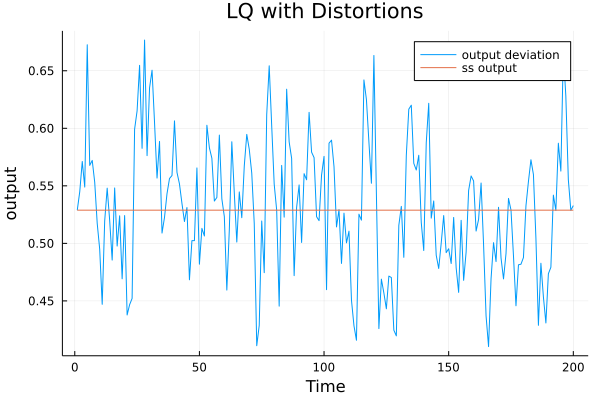
\includegraphics[width=1\textwidth]{y_dev_LQ_new.png} % first figure itself
        \caption{Output deviation: LQ}\label{y_compLQ}
    \end{minipage}\hfill
    \begin{minipage}{0.45\textwidth}
        \centering
        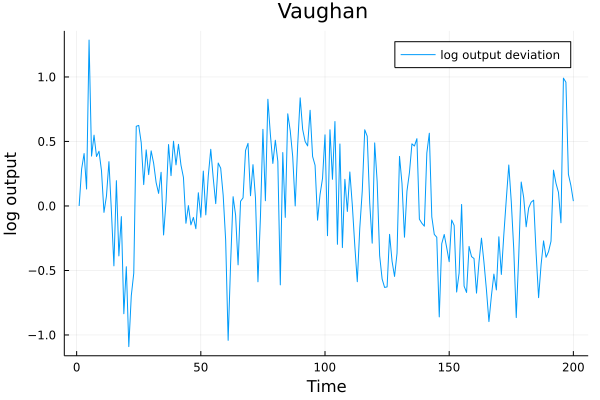
\includegraphics[width=1\textwidth]{log_y_dev_vaughan_new.png} % second figure itself
        \caption{Log Output deviation}\label{y_compV}
    \end{minipage}
\end{figure}
As we can see the output deviation graphs are very close to each other verifying that both the methods give the same answer.


\section{Accounting Profits and Stock Valuation}
We use the following formula to calculate the dividends, accounting profits, and stock valuation. 
\begin{align*}
A_{pt} = F(k_t, h_t, z_t) - \delta k_t \\
\tilde{A}_{pt} = \frac{\theta y_{ss}[\theta \tilde{k}_t + (1-\theta)(\tilde{h}_t + \tilde{z}_t)] - \delta k_{ss} \tilde{k}_t}{A_{pss}} \\
D_t = \theta k_t^{\theta}(h_t z_t)^{1-\theta} -(\tilde{\gamma} + (1-\delta)k_{t+1} -(1-\delta)k_t) - \tau_{pt}A_{pt} \\
S_t = (1-\tau_{dt})k_t.
\end{align*}

\subsection{Discussion of Results}
We note from the preceding figures that Accounting profits and Stock valuation are strongly positively correlated. The deviation in consumption and hours worked in inversely related. Further, the stock valuation is more smooth compared to other fluctuations.

\subsection{Example}
In the following example we keep only the government wedge and shut down all other channels. The output deviation in the case with government wedge is lower than without the government wedge. This example is interesting since it shows that government expenditure may reduce output volatility.
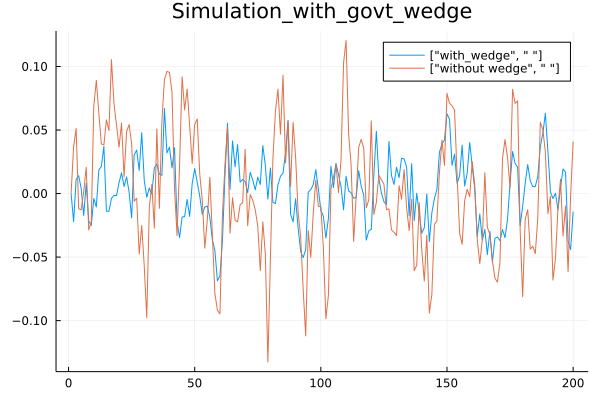
\includegraphics[scale=0.5]{figure5.png} % first figure itself


%\newpage
%\bibliography{ref}

\end{document}